\documentclass[12pt]{article}
\usepackage{amsmath}
\usepackage[T1]{fontenc}
\usepackage{graphicx}
\usepackage{amsfonts}
\usepackage{tikz}
\usepackage{listings}
\newcommand{\floor}[1]{\left\lfloor #1 \right\rfloor}	% podłoga
\newcommand{\ceil}[1]{\left\lceil #1 \right\rceil}		% sufit
\newcommand{\fractional}[1]{\left\{ #1 \right\}}		% część ułamkowa {x}
\newcommand{\abs}[1]{\left| #1 \right|}					% wartosc bezwzgledna / moc
\newcommand{\set}[1]{\left \{ #1 \right \}}				% zbiór elementów {a,b,c}
\newcommand{\pair}[1]{\left( #1 \right)}				% para elementów (a,b
\title{AISD lista 5}
\author{Dominik Szczepaniak}
\begin{document}

\maketitle

\bgroup\obeylines

\section{Zadanie 1}
Model drzew decyzyjnych to model porównywania wartość a jest mniejsza od wartości b.\\

Czyli w takim razie żeby problem znajdowania otoczki wypukłej był możliwy do rozwiązania w tym modelu to musimy być w stanie jednoznacznie powiedzieć kiedy punkt jest na otoczce wypukłej.\\

Weźmy sobie punkty $W1 = (1, 4), W2 = (1, 1), W3 = (3, 1)$
Rozpatrzmy dodatkowo punkt $P1 = (2, 2.5)$ - w tym przypadku otoczka wypukła zrobiona na W1, W2 i W3 zawiera w sobie punkt P1.
Niech $P2 = (2.5, 2.9)$
W tym przypadku punkt P2 leży poza otoczką wypukłą zbudowaną na punktach W1, W2 i W3, więc musimy rozszerzyć otoczkę wypukłą o ten punkt. \\

No ale zauważmy, że dla obu punktów zachodziły dokładnie te same nierówności względem wszystkich 3 punktów, więc oba przypadki są nierozróżnialne, mimo iż mają inne rozwiązania, więc problemu znajdowania otoczki wypukłej nie można rozwiązać w modelu drzew decyzyjnych.

\section{Zadanie 2}
Udowodnij, że omega(nlogn) jest dolnym ograniczeniem dla problemu 3SUM w modelu drzew decyzyjnych.\\

Aby to udowodnić chcemy zrobić liniowe drzewo decyzyjne i pokazać, że wszystkie odpowiedzi wpadają do jakiegoś liścia w tym drzewie. \\

Nasze liczby $\set{x_1, x_2, ..., x_n}$ możemy traktować jako punkt w przestrzeni $R^n$.
W drzewach decyzyjnych mogliśmy porównywać dwie liczby, w liniowych drzewach decyzyjnych porównujemy kombinacje liniowe danych na wejściu. \\

W przypadku tego zadania chcemy skorzystać z liniowych drzew decyzyjnych - drzew tryarnych, w których mamy trzy przyrównania - mniejsze, większe i równe. W wierzchołkach mamy kombinacje liniowe elementów ciągu wejściowego. Czyli za każdym razem dzielimy naszą przestrzeń przeszukiwań hiperpłaszczyznami i patrzymy czy jesteśmy poza tą płaszczyzną i z której strony czy na niej. \\

Idea jest taka, że chcemy stworzyć liniowe drzewo decyzyjne i dużo istancji problemów, rzędu n! i pokazać, że odpowiedź na każdy z tych problemów jest w jakimś liściu. \\

Z dowodu z wykładu mamy:
Niech $T_n = (V, E)$ będzie liniowym drzewem decyzyjnym dla rozważanego problemu ograniczonego do danych $R^n$. Dla każdego wierzchołka $v \in V$ przez S(v) oznaczamy zbiór tych punktów z $R^n$ które osiągają v. 
Dla każdego $v \in V$ zbiór S(v) jest wielościanem wypukłym.\\

Jak stworzyć dużo instancji problemów, które będą w liściach. 
$P_1, P_2, ...$ są różnymi punktami z $R^n$. 
Tworzymy instancje tych problemów, tak, że bierzemy odpowiednio liczby:
$P=1, 3, 5, ..., n-1, 2*n, -(2n+2), -(2n + 4), ..., -(2n + n-1)$
Bierzemy takie liczby, ponieważ za chwilę pokażemy, że nie ma dla nich wyniku, więc w ostateczności trzeba by było przejrzeć je wszystkie i dla każdych trzech wylądują potencjalnie w innym liściu.
Mamy więcej podproblemów niż tylko P. Skupiamy się na podproblemach P i próbujemy je od siebie odróżniać. Wychodzimy poza rodzinę problemów P, bo jednak mówię, że jest tam podproblem, którego rozwiązanie da odpowiedź "tak".

DLACZEGO ODPOWIEDŹ DLA KAŻDEJ INSTANCJI TEGO PODPROBLEMU BRZMI "NIE":
- potrzebujemy przynajmniej jednej ujemnej liczby, ponieważ suma trzech dodatnich liczb nie da nam zera. W takim razie weźmy najmniejszą liczbe ujemną i dwie największe liczby dodatnie (na razie nie rozważamy 2n). W takim przypadku mamy $n-1 + n-3 + (-2n+2) = 2n - 4 - 2n - 2 = -6 != 0$. Liczby dodatnie są tylko i wyłącznie mniejsze, a liczby ujemne również maleją dlatego nie możliwe jest dobranie jakichkolwiek parametrów tak, aby zniwelować różnicę między ich sumą. 

- dochodzimy do wniosku, że na pewno musimy skorzystać z 2n. Ale w momencie dodania do liczby 2n jakiejkolwiek liczby ujemnej np. 2n + (-(2n+2)) = -2. W zbiorze liczb dodatnich, którymi dysponujemy znajdują się jedynie liczby nieparzyste, zatem nie jesteśmy w stanie znaleźc składnika, który doprowadzi nas do wyniku 0. 

A więc mamy $\frac{n}{2}!$ różnych podproblemów na które odpowiedź na pewno brzmi "NIE". \\

Następnym krokiem jest pokazanie, że każda z tych odpowiedzi ląduje w innym liściu. (drzewo ma tyle liści co podproblemów). \\

Załóżmy niewprost, że odpowiedzi są w tym samym liściu.
Weźmy dowolne punkty $P_i, P_j$ takie, że różnią się na k-tej współrzędnej. Załóżmy, że nie znajdują sie one w tym samym liściu. Jeżeli tak jest, to są na tej samej hiperpłaszczyźnie, więc na linii między $P_i$ a $P_j$ wszystkie punkty należą do tej płaszczyzny czyli dają taką samą odpowiedź NIE. Zatem istnieje jakiś punkt P między nimi, który na k-tej współrzędnej ma liczbę parzystą. Weźmy go zatem. \\

Ale skoro ma on liczbe parzystą na k-tej pozycji, to algorytm powinien zwracać dla niego "tak", bo P(k) + 2n + -(2n + P(k)) = 0. Wiemy, że -(2n + P(k)) należy do naszego zbioru danych, bo skoro ten punkt leży między $P_i$ a $P_j$ to też 1 < k < n. Stąd sprzeczność.\\

A więc mamy $\frac{n}{2}!$ liści. Więc: $(h_n to wysokość drzewa)$
$3^{h_n} \geq \frac{n}{2}!$
$h_n \geq log_3(\frac{n}{2}!) \geq c * n * log_2{n}$

\section{Zadanie 3}

1. Wrzucamy wszystko do hashmapy
2. przechodzimy dwoma wskaznikami i i j po tablicy i pytamy czy -(S[i] + S[j]) jest w hashmapie
===============================
Algorytm używający dwóch pointerów:

Najpierw sortujemy nasza tablice.
Pozniej idziemy forem i bierzemy sobie ten element na ktorym jestesmy jako jeden z 3 elementow.
Pozostale dwa elementy j, k ustawiamy bazowo na i+1 oraz n-1 (gdzie i to indeks elementu z fora)
Pozniej whilem dopoki j < k 
Jesli s[i] + s[j] + s[k] = 0 to mamy wynik wypisujemy tak
wpp jesli sa wieksze od 0 to zmniejszamy k 
jesli sa mniejsze od 0 to zwiekszamy j

Dlaczego działa?
Załóżmy, że mamy rozwiązanie a+b+c=0. Poniewaz pointery ruszają się tylko w jedną strone mozemy zalozyc, ze glowny pointer z petli wybierze nam kiedys a, a pozniej idac pointerem j albo k znajdziemy b lub c (ktorys z nich musimy znalezc), a wtedy algorytm bedzie schodzil drugim pointerem do c lub b i otrzymamy trojke - a, b, c.

\begin{lstlisting}
    sort(S);
    for i = 0 to n - 2 do
        a = S[i];
        start = i + 1;
        end = n - 1;
        while (start < end) do
            b = S[start]
            c = S[end];
            if (a + b + c == 0) then
                output a, b, c;
                // Continue search for all triplet combinations summing to zero.
                // We need to update both end and start together since the array values are distinct.
                start = start + 1;
                end = end - 1;
            else if (a + b + c > 0) then
                end = end - 1;
            else
                start = start + 1;
        end
    end
\end{lstlisting}

\section{Zadanie 4}
Jeśli obliczymy wszystkie pary xorów to mamy $O(n^2)$. 
Zapiszmy wszystkie elementy w hashmapie lacznie z ich indeksami
Przechodzimy dwoma wskaznikami po tablicy i oraz j i pytamy czy S[i] xor S[j] jest w hashmapie i nie jest ani i ani j. 
Jeśli tak to mamy odpowiedź, bo xor dwóch takich samych elementów jest równy 0. 

To rozwiązanie jest na ogół w złożoności $O(n^2)$, ale z tego jak działa hashmapa, wiemy, że ma ona średni czas dostępu O(1), ale mogą być takie przypadki, że czas dostępu będzie O(n), jeśli ktoś wyliczy takie wejście, że hashe będą wpadać do tych samych kubełków.
=================================
W takim razie jak dostać rozwiązanie które ma złożoność dokładnie $O(n^2)$, niezależnie od wejścia?
Zauważmy, że rozwiązanie 3SUM działało, ponieważ mieliśmy wszystko posortowane i zachodziło, że możemy chodzić dwoma wskaźnikami po tablicy. W xorze niestety nie zachodzi a xor x < a xor y dla x < y. Możemy zrobić za to sortowanie leksykograficznie rosnące, które spowoduje, że własność będzie zachodzić. 



1. Posortujmy sobie nasze wejście O(nlogn)
2. Robimy sobie specjalnie BST ktore umozliwia dla dowolnego ciagu 0 i 1 przejsc zbior $a xor X = {a xor x | x \in X}$ w ciagu leksygograficznym rosnacym w czasie $O(|X|)$.

Jak tworzymy nasze drzewo?
\begin{enumerate}
    \item Jeśli $X = {x}$ to $T_x$ jest liściem - LeafNode(x) 
    \item Jesli $|X| \geq 2$ to przez $lcp(X)$ oznaczymy najdluzszy wspolny prefiks wszystkich elementow z X oznaczanych jako ciagi 0 i 1. Oznaczmy przez $T_x = InnerNode(T_{X_0}, 0^k1b, T_{X_1})$, dla jakiegoś b = ${0, 1}^{w-k-1}$ -> drzewo $T_x$ składa się z korzenia z wartością $0^k1b$, lewym poddrzewem $T_{X_0}$ oraz prawym poddrzewem $T_{X_1}$. Wybór b jest nieważny, ważne jest aby $l = (max X_0) xor (max X_1)$. \\ Zauważmy, że ścieżki z korzenia są malejące jeśli zamienimy ciągi 0, 1 na liczby w systemie dziesiętnym. 
\end{enumerate}



Algorytm:
\begin{lstlisting}
    def MakeTree(X):
        sort(X) as x1 < ... < xn
        let l_i = x_i xor x_i+1 1 <= i < n
        stream = (inf, x_1, l_1, x_2, l_2, ..., l_n-1, x_n, inf)
        return build()
        def build(){
            l = pop(stream)
            x = pop(stream)
            T = LeafNode(x)
            while(top(stream) < l){
                l' = top(stream)
                T = InnerNode(T, l', build())
            }
        }

    def traverse(T, a){ - dla drzewa T = T_X i a w X zwraca zbior {a xor x | x in X} w porzadku rosnacym
        if T == LeafNode(x){
            yield a xor x;
        }
        else{
            let T = InnerNode(T_0, l, T_1)
            if a xor l > a{
                traverse(T_0, a);
                traverse(T_1, a);
            }
            else{
                traverse(T_1, a);
                traverse(T_0, a);
            }
        }

    }

    def 3XOR(X):
        sort(X) x1 < ... < xn;
        TX = MakeTree(X)
        for a in X{
            (i, j) = (1, 1)
            (y_i) 1<=i<=n = traverse(TX, a)
            while i<=n and j<=n{
                if y_i < x_j{
                    i++;
                }
                else if(y_i > x_j){
                    j++;
                }
                else{
                    return "TAK" (a, y_i xor a, x_j)
                }
            }
        }
        return "NIE"
\end{lstlisting}

Dowód poprawności:

\section{Zadanie 5}
Szukamy w zbiorze $\set{x_1, x_2, ..., x_n}$ takich punktów, że trzy z nich są współliniowe.

Oznaczmy nasze punkty przez $A = (x_1, y_1), B = (x_2, y_2) oraz C = (x_3, y_3)$
Trzy punkty są współliniowe jeśli pole trójkąta utworzonego przez te punkty jest równe zero, co można wyrazić za pomocą równania macierzowego:

\begin{equation}1/2 * \text{det} \left(\begin{array}{ccc}x_1 & y_1 & 1 \\x_2 & y_2 & 1 \\x_3 & y_3 & 1 \\\end{array}\right) = x_1(y_2 - y_3) + x_2(y_3 - y_1) + x_3(y_1 - y_2) = 0\end{equation}
Wyznacznik ten można przekształcić do postaci:
\begin{equation}1/2*(x_1(y_2 - y_3) + x_2(y_3 - y_1) + x_3(y_1 - y_2)) = 0\end{equation}
Ponieważ 1/2 nas nie obchodzi (bo przyrównujemy do 0) to szukamy tylko tych rzeczy w środku nawiasu.

W takim razie znowu chcemy znaleźć trzy punkty takie, że ich suma jest równa zero. Nasza różnica między tym problemem, a problemem 3SUM polega na tym, że w tym problemie nasze punkty są w $R^2$, a w 3SUM w $R^1$. Ponieważ nasza logika polegała na reprezentowaniu ciągu wejściowego punktów jako punktu w $R^n$, to tutaj mamy punkt w $R^2N$, a nasza dalsza logika jest taka sama. Stąd wynika, że jeśli ten problem rozwiążemy w czasie $O(n^{2-\epsilon})$ to rozwiążemy też 3SUM w czasie $O(n^{2-\epsilon})$.

=====================

Przejdźmy z 3SUM do tego problemu:
Dla każdej liczby w zbiorze 3SUM wyznaczmy punkty jako $(x, x^3)$. Zbadajmy kiedy otrzymane 3 punkty $(a, a^3), (b, b^3), (c, c^3)$ są współliniowe:
$\frac{b^3-a^3}{b-a} = \frac{c^3-b^3}{c-b} \Rightarrow \frac{(b-a)(b^2+ab+a^2)}{b-a} = \frac{(c-b)(c^2+bc+b^2)}{c-b} \Rightarrow a^2+ab+b^2 = b^2+bc+c^2 \Rightarrow a^2-c^2+ab-bc = 0 \Rightarrow (a-c)(a+c) + b(a-c) = 0 \Rightarrow (a-c)(a+b+c) = 0 \Rightarrow a+b+c = 0$

\section{Zadanie 6}

Chcemy scalić dwa n elementowe ciągi $A = a_1, a_2, ..., a_n$ i $B = b_1, b_2, ..., b_n$ w jeden posortowany ciąg $X$. Zakładamy, że ciągi $A$ oraz $B$ są posortowane (inaczej scalanie nie miałoby sensu). 
Cała przestrzeń danych, czyli wszystkie możliwe ustawienia ciągu $X$ to ${2n}\choose{n}$, bo wybieramy $n$ z $2n$ miejsc na jeden ciąg, a pozostałe wypełniamy drugim. 
Adwersarz ogranicza przestrzeń danych, tak aby zawierała $2n$ zestawów danych. 

Strategia adwersarza będzie opierać się na warunku:
$a_1<b_1<a_2<b_2<a_3<b_3<a_4<b_4<...<a_n<b_n$

Zapiszmy nasz ciag jako zestaw $2n-1$ par stworzonych z sąsiadujacych ze sobą elementów, czyli takich, które możemy zamienić miejscami bez utraty poprawności strategii adwersarza.
 $<(a_1, b_1), (b_1, a_2), (a_2, b_2)\dots, (a_k, b_k), (b_k, a_{k+1}), (a_{k+1}, b_{k+1})\dots,(a_n, b_n)>$
 
 Zauważmy, że mamy $2n$ możliwych ciągów, ponieważ możemy zamienić elementy w każdej z $2n-1$ par lub nie zamienić w żadnej.
 
 Zakładamy, że gracz nie zadaje głupich tzn. nie dających mu nowych informacji pytań. Wie, że ciągi A i B były posortowane, wiec $a_i<a_{i+1}$ i $b_i<b_{i+1}$.
 
 Rozważmy wszytskie pytania jakie może zadać gracz i pokażmy, że każde z nich eliminuje co najwyżej jeden zestaw danych. Wówczas wykażemy, że do scalenia dwóch posortowanych podciągów potrzebne jest conajmniej 2n-1 porównań.
 // i bedzie indeksem dla a, j dla b
 
 1) $i>j+1$ adwresarz odpowie,że $b_j<a_i$. Nie zmiejsza to ilości zestawów/ciągów, bo $a_i$ i $b_j$ nie są w tej samej parze.
 
 2) $i=j+1$ adwresarz odpowie,że $b_j<a_i$ i wyeliminuje jeden ciąg, taki w którym była zamieniana para $(a_i, b_j)$, czyli $(b_j, a_{j+1})$  np. $(b_1, a_2)$
 
 3) $i<j$ adwresarz odpowie,że $a_i<b_j$. Nie zmiejsza to ilości zestawów/ciągów, bo $a_i$ i $b_j$ nie są w tej samej parze.

 4) $i=j$ adwresarz odpowie,że $a_i<b_j$ i wyeliminuje jeden ciąg, taki w którym była zamieniana para $(a_i,b_j)$, czyli $(a_i, b_i)$
 
Widzimy, że każde zapytanie usunie co najwyżej jeden zestaw. 

**PRZYKŁAD**
$n = 2$
$<(a_1, b_1)(b_1, a_2)(a_2, b_2)>$
Otrzymujemy z tego ciągi:
$a_1, b_1, a_2, b_2$ - nie zamieniamy żadnej pary
$b_1, a_1, a_2, b_2$ - zamieniamy pierwszą parę miejscami
$a_1, a_2, b_1, b_2$ - zamieniamy środkową parę
$a_1, b_1, b_2, a_2$ - zamieniamy ostatnią parę

\section{Zadanie 7}

\section{Zadanie 8}
% https://gist.github.com/rcyeh/8ba1d5df3932ce7fb22070a23d321b0b

https://www.cs.cmu.edu/~ckingsf/bioinfo-lectures/3dm.pdf

Robimy sobie kółko "gadgetów" które mają dwie warstwy - wewnętrzne kółko oraz zewnętrzne kółko.
Dla każdej zmiennej tworzymy 2 nowe zmienne $y_{c_1}$ oraz $z_{c_1}$. Zauważmy, że tylko dla jednej trójki zmiennych (klauzul) używamy $y_{c_1}$ oraz $z_{c_1}$, więc tylko jedna z tych klauzul znajdzie się w rozwiązaniu. Wybrana trójka (z $y_{c_1}$ oraz $z_{c_1}$) jest tą trójką która wybiera która wartość była prawdziwa. \\
Klauzule:
Dla przykładu. Jeśli mamy formułę $x_{i_1} \lor x_{j_1} \lor \lnot x_{k_1}$ to stworzymy:
$y_{i_1} \lor z_{j_1} \lor x_{i_1}$ oraz $z_{i_1} \lor y_{j_1} \lor x_{j_1}$ oraz $z_{i_1} \lor y_{j_1} \lor \lnot x_{k_1}$  
Więc teraz w 3D matchingu możemy wybrać tylko jedną z tych klauzul, bo inaczej nie będzie spełniona własność 3D matchingu.\\

Zmienne:
Możemy to ugólnić:
Załóżmy, że $b_i$ oraz $\lnot b_i$ pojawiają się n razy w klauzulach.
Wtedy robimy:
1. Tworzymy 2n nowych zmiennych $y_{i_1}$ do $y_{i_n}$ oraz $z_{i_1}$ do $z_{i_n}$
2. Tworzymy 2n nowych trójek:
$(b_{i_1}, y_{i_1}, z_{i_1})$, $(b_{i_2}, y_{i_2}, z_{i_2})$,...,$(b_{i_n}, y_{i_n}, z_{i_n})$
$(\lnot b_{i_1}, y_{i_1}, z_{i_1})$, $(\lnot b_{i_2}, y_{i_2}, z_{i_2})$,...,$(\lnot b_{i_n}, y_{i_n}, z_{i_n})$
3. Zauważmy:
- Każda $y_i$ oraz $z_i$ pojawia się tylko w jednej z dwóch trójek ($b_i$ oraz $\lnot b_i$) 
- Przez strukturę koła albo wszystkie trójki z $b_i$ są w rozwiązaniu albo wszystkie trójki z $\lnot b_i$ są w rozwiązaniu. 
- Dla tego kółka trójki w rozwiązaniu są tymi które nie powodują, że klauzula jest prawdziwa. Dzieje się tak, ponieważ trójki włożone do zbioru rozwiązania ze zmiennych, są niedostępne.\\

Mamy teraz rozwiązanie 3SAT za pomocą 3D matchingu. Problemem jest to, że niektóre zmienne w ogóle nie są użyte, więć musimy się jakoś tym zająć, bo inaczej nie będzie to 3D matching.\\



Musimy stworzyć sobie kilka nowych wierzchołków. Nasze zmienne $b_i$ oraz $\lnot b_i$ są zmiennymi pochodzącymi z X, a $y_i$ oraz $z_i$ są zmiennymi pochodzącymi z Y oraz Z. Musimy zagwarantować, że wszystkie wierzchołki będą użyte, więc stworzymy $n_i$ wierzchołkow, gdzie $n_i$ to liczba klauzul zawierających dodatkowe y i z wierzchołki z dodatkowymi b-zmiennymi. Robimy ten "garbage collector" n - ilość klauzul razy.\\

===================================\\
PRZYKŁADY:
$(p \lor q \lor r) \land (\lnot p \lor \lnot q \lor \lnot r)$

Klauzule:
$(p \lor y_{c_1} \lor z_{c_1})$, $(q \lor y_{c_1} \lor z_{c_1})$, $(r \lor y_{c_1} \lor z_{c_1})$
$(\lnot p \lor y_{c_2} \lor z_{c_2})$, $(\lnot q \lor y_{c_2} \lor z_{c_2})$, $(\lnot r \lor y_{c_2} \lor z_{c_2})$

Zmienne:
$(p, y_{p_1}, z_{p_1})$, $(\lnot p, y_{p_1}, z_{p_1})$
$(q, y_{q_1}, z_{q_1})$, $(\lnot q, y_{q_1}, z_{q_1})$
$(r, y_{r_1}, z_{r_1})$, $(\lnot r, y_{r_1}, z_{r_1})$

Dodatkowe wierzchołki:
$(p, y_{g_1}, z_{g_1})$, $(\lnot p, y_{g_1}, z_{g_1})$, $(q, y_{g_1}, z_{g_1})$, $(\lnot q, y_{g_1}, z_{g_1})$, $(r, y_{g_1}, z_{g_1})$, $(\lnot r, y_{g_1}, z_{g_1})$
T ma 18 trójek; n = 6

Jeden z poprawnych subsetów S ma 
$(p, y_{c_1}, z_{c_1}), (\lnot q, y_{c_2}, z_{c_2}), (\lnot p, y_{p_1}, z_{p_1}), (q, y_{q_1}, z_{q_1}), (\lnot r, y_{r_1}, z_{r_1}), (r, y_{g_1}, z_{g_1})$

Co mówi o $p = true, q = false, r = true$
(prawdziwe wartości są w klauzulach i dodatkowych wierzchołkach)

\section{Zadanie 9}
WYSTARCZY:
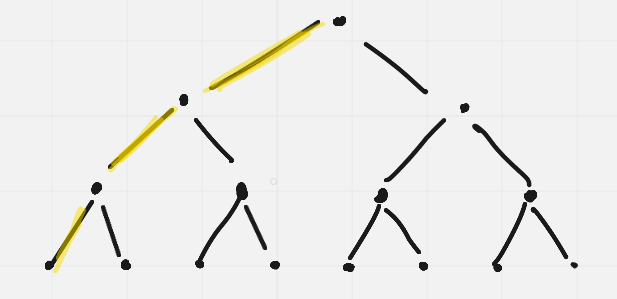
\includegraphics[scale=0.5]{zad6_1.png}
Rozwiązaniem zadania jest drzewo decyzyjne.
Aby wybrać element wygrywając i doprowadzić go do korzenia drzewa należy wykonać $n - 1$ porównań.
Aby wybrać drugi element największy należy wybrać go z pośród elemetnów które przegrały ze zwycięzcą (największym elementem).
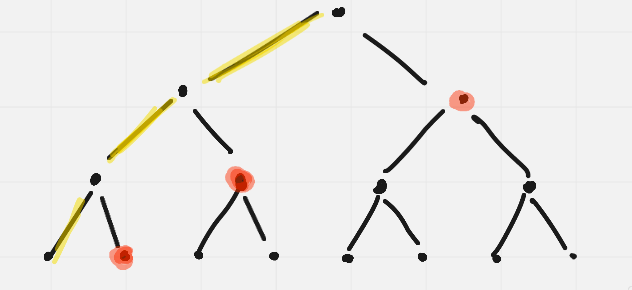
\includegraphics[scale=0.5]{zad6_2.png}
Takich elementóe jest $log\ n$ (wysokość drzewka o n liściach to $log\ n$).
Aby znaleźć największe z nich należy dokońać $log\ n - 1$ porównań.

$n - 1 + \log n - 1 = n + \log n - 2$

$\newline$

POTRZEBA (nie da się mniejsza ilością porównań uzyskać odpowiedzi):

Wy wyniku działania powyższego algorytmu dzielimy zbiór n-elemetnowy na element największy - MAX1, element drugi największy - MAX2 i zbiór pozostałych clementów, których jest n-2.

Rozważmy problem znalezienia n-2 elementów mniejszych od drugiego największego elemetnu MAX2.

Wiemy, że aby stwierdzić, że element jest mniejszy od MAX2 musimy go z nim porównać lub porównać go z elementem, który wiemy, że jest mniejszy niż MAX2.
Takich porównań będzie n-2.

Teraz wystarczy, że pokażemy, że aby znaleźć MAX1 wykonaliśmy $\log n$ porównań.

Wprowadźmy oznaczenie:
niech $L(x)$ oznacza liczność zbioru składającego się elementów mniejszych lub równych x  (które ustaliliśmy, że takie są w trakcie trwania algorytmu)

Jeśli porównujemy dwie liczby x i y, to gdy $x \leq y$ to $L(x) \leq L(y)$ ( y jest większe, więc będzie więcej elementów mniejszych od y)

Czyli skoro $x\leq y$ to $L(y) = L`(y) + L(x)$ (kolejne "wywołania algorytmu")
Czyli z każdym porównaniem $L(y)$ może powiększyć się maksymalnie dwukrotnie (, bo gdy $x \leq y$ to $L(x) \leq L(y)$)
Czyli po k porównaniach mamy $L(y) \leq 2^k$, bo na początku mamy $L(y) = 1$ ( na poczatku wiemy tylko, że y jest mniejszy lub równy y)

$L(MAX1)= n$ bo MAX1 jest maximum zbioru
stąd:
$L(MAX1)=n \leq 2^k$ //logarytmujemy
$logn \leq k$ gdzie k to liczba porównań
$\lceil logn \rceil \leq k$, bo k to liczba całkowita

Stąd potrzebujemy $\lceil logn \rceil+n-2$ porównań.

\egroup
\end{document}